\subsection{The Background Subtractor}
\label{subsection:training}
The background subtractor is reposible for determining which pixels are background and which are foreground objects. The subtractor uses a Mixture of Gaussian model (section \ref{subsection:mog}) to cluster the pixels into those two sets - background and forground. Initially the model is 'trained' on several hundred images - a few seconds of video - so that it's immediate use yields the most accuracte statistics. The software implemntation of a Gaussian mixture model used is OpenCV's BackgroundSubtractorMOG2 function \cite{opencv_mog2}. This implementation is based on the research by Zoran Zivkovic and Ferdinand van der Heijden \cite{zivkovic_pattern_recognition} \cite{zivkovic_heijden_pattern_recognition_letters} in which a method of using a Gaussian Mixture Model (GMM) that improves upon former GMM in both speed and effectiveness at segmenting foreground objects, taking only a pixel's intensity as a feature. The subtraction component of the detection process was by far the most complex and thus the most computationally expensive, requiring each pixel in an image to have it's own probability density distrubtion and then to recalculate that for each new image. It was imperative, however, that the algorithm be fast enough that images could be processed as they arrived in real-time so that traffic data could reflect live conditions. Fortunately the speed of this implementation made it a suitable fit for a low power microcontroller and it's effectiveness ensured it's adoption into the system, as can be seen in Figure \ref{fig:example_subtraction}. This method is particularly effective at picking up moving objects as they cause pixels to have constantly changing intensities and making it easy for the model to determine that they're not a part of the background. 

Notice in Figure \ref{fig:foreground_mask_filtered} the gray pixels in and around the foreground objects, these are shadows that the OpenCV's GMM implemetation can explicitly detect. They are removed by thresholding (equation \ref{eq:threshold}) values that are not white and converting them to black (background) pixels.

\begin{figure*}[htbp]
    \centering 
    \begin{subfigure}[b]{0.45\textwidth}
        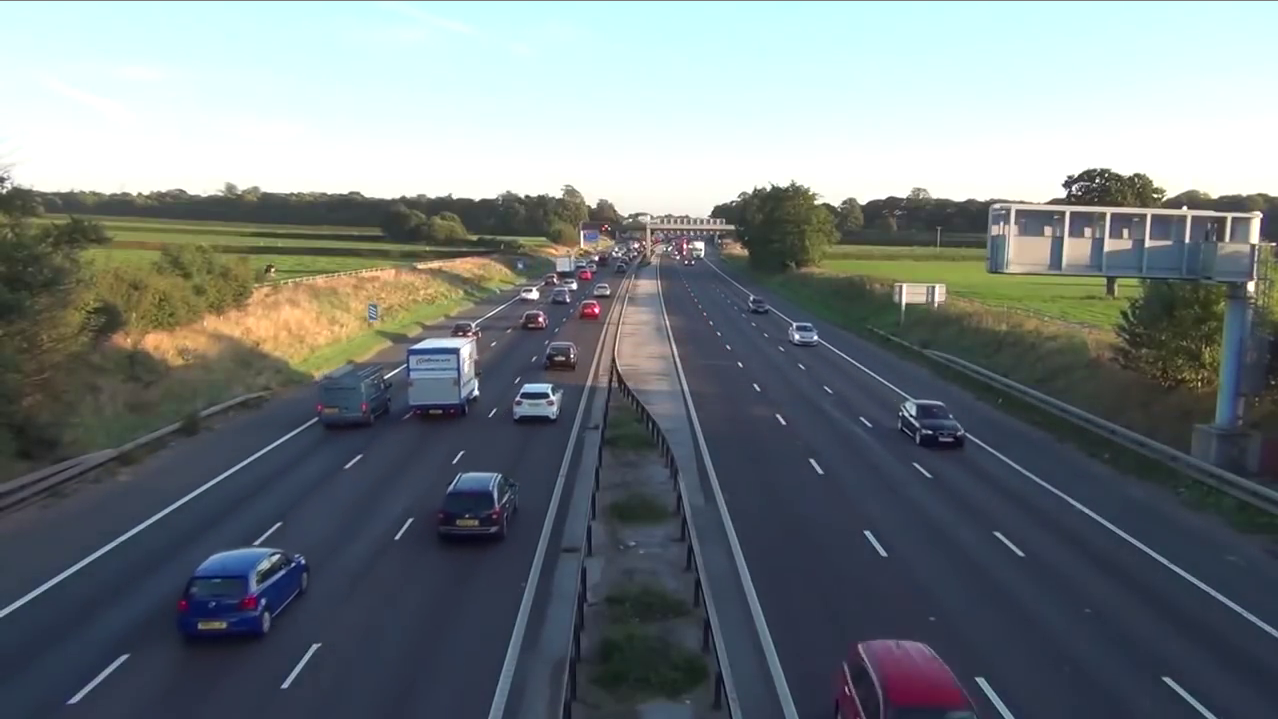
\includegraphics[width=\textwidth]{design/detection/subtractor/original_frame}
        \captionsetup{format = hang}
        \caption{The original frame of traffic. Img: Andrey Nikishaev.}
        \label{fig:original_frame}
    \end{subfigure}
    \begin{subfigure}[b]{0.45\textwidth}
        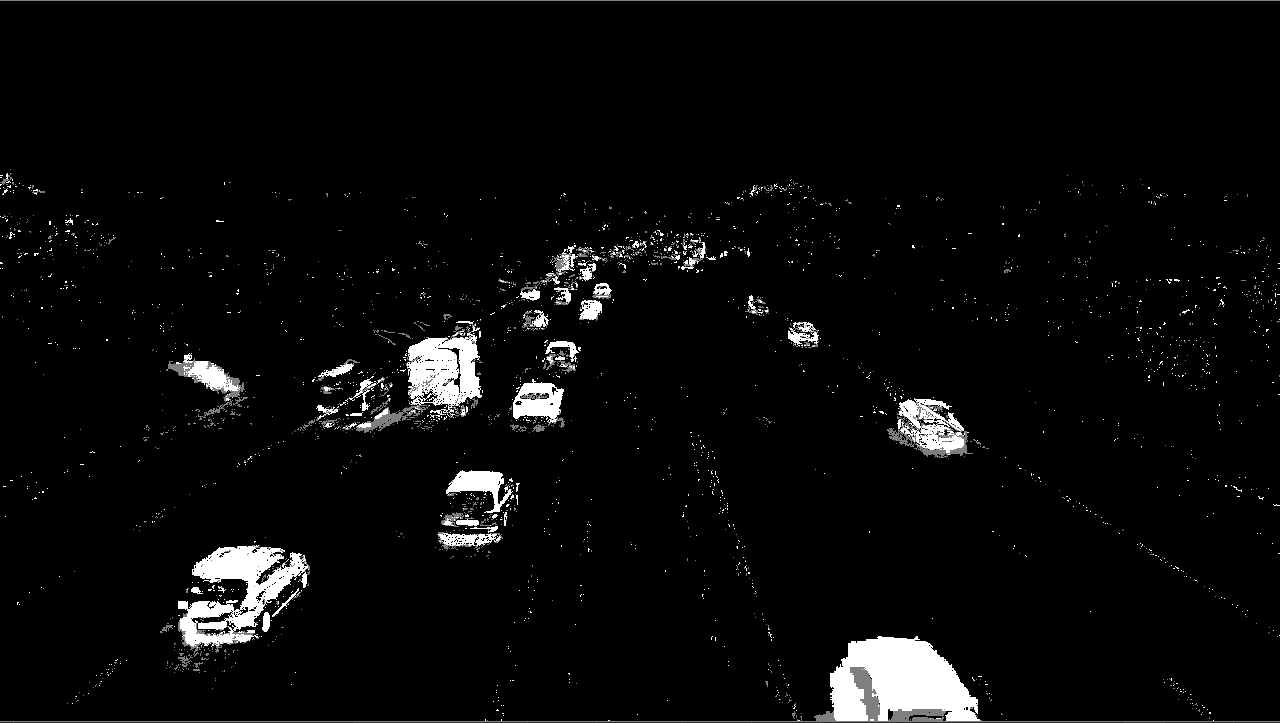
\includegraphics[width=\textwidth]{design/detection/subtractor/foreground_mask}
        \captionsetup{format = hang}
        \caption{Foreground mask generated by GMM clustering.}
        \label{fig:foreground_mask_unfiltered}
    \end{subfigure}
    \captionsetup{format=hang}
    \caption{A foreground mask generated from a traffic scene by OpenCV's GMM implementation.}
    \label{fig:example_subtraction}
\end{figure*}